\documentclass{beamer}
\usepackage[utf8]{inputenc}
\usepackage{listings}
\usepackage{multicol}
\usepackage{graphicx}
\usepackage{caption}

\usetheme{Frankfurt}
\usecolortheme{default}


\title[Crisis]{Introduction to contract programming}
\author{Łukasz Ziobroń}
\institute{Nokia}
\date{Code Dive Community, 2015}
\subject{Computer Science}
\lstset
{
    language=C++,
    numbers=left,
    basicstyle=\ttfamily\scriptsize,
    keywordstyle=\color{blue}\ttfamily,
    stringstyle=\color{red}\ttfamily,
    commentstyle=\color{green}\ttfamily,
}
\graphicspath{ {./img/} }
\DeclareGraphicsExtensions{.pdf,.png,.jpg}
\DeclareCaptionFormat{listing}{\vskip1pt#1#2#3}
\captionsetup[lstlisting]{format=listing,singlelinecheck=false}



\begin{document}


\begin{frame}
\titlepage
\end{frame}

\begin{frame}
\frametitle{Table of Contents}
\begin{multicols}{2}
\tableofcontents
\end{multicols}
\end{frame}


\section{Some examples}
\subsection{Ariane 5 mission}
\begin{frame}
\frametitle{Ariane 5 mission}
\only<1>
{
  In 1996, the Ariane 5 rocket was reusing software from the Ariane 4. 37 seconds after its maiden launch the self-destruct safety mechanism was activated. \\~\\
  A data conversion from 64-bit floating point value to 16-bit signed integer value to be stored in a variable representing horizontal bias caused a processor trap because the floating point value was too large to be represented by a 16-bit signed integer. \footnote{https://en.wikipedia.org/wiki/Ariane\_5\#Notable\_launches} \\~\\
  This bug, existing in Ariane 4 software never came out on Ariane 4 rocket.
}
\only<2>{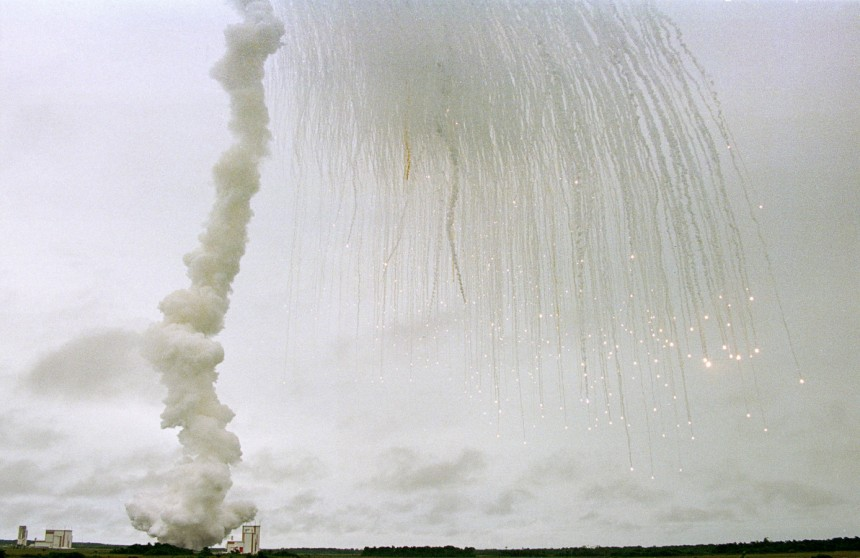
\includegraphics[scale=0.35]{ariane}}
\end{frame}

\subsection{Calculator source code}
\begin{frame}[fragile]
\frametitle{Basic calculator}
\only<1>{ \lstinputlisting[linerange={26-36}]{"src/calculator.cpp"} }
\only<2>{ \lstinputlisting[linerange={38-60}]{"src/calculator.cpp"} }
\only<3>{ \lstinputlisting[linerange={62-74}]{"src/calculator.cpp"} }
\only<4>{ \lstinputlisting[linerange={76-88}]{"src/calculator.cpp"} }
\end{frame}

\subsection{Blender interface}
\begin{frame}[fragile]
\frametitle{Blender interface}
\only<1>{ \lstinputlisting[linerange={26-36}]{"src/Blender.java"} }
\end{frame}


\section{DbC Theory}
\subsection{What is a contract?}
\begin{frame}
\frametitle{What is Contract by Design?}
\setbeamercovered{transparent}
\uncover<1-2>{A paradigm which was first introduced by Bertrand Meyer, the creator of Eiffel. Although Eiffel has support for programming by contract built into the language, most of the concepts can be used in any language \footnote{http://www.cs.unc.edu/~stotts/COMP204/contract.html}.  \\~\\}
\uncover<2-2>{Basically programming by contract creates a contract between the software developer and software user - in Meyer's terms the supplier and the consumer.  \\~\\}
\end{frame}

\subsection{3 assumptions}
\begin{frame}
\frametitle{3 assumptions}
\setbeamercovered{transparent}
\uncover<1-3>{Every feature, or method, starts with a \textbf{precondition} that must be satisfied by the consumer of the routine. \\~\\}
\uncover<2-3>{And each feature ends with \textbf{postconditions} which the supplier guarantees to be true (if and only if the preconditions were met). \\~\\}
\uncover<3-3>{Also, each class has an \textbf{invariant} which must be satisfied after any changes to the object represented by the class. In the other words, the invariant guarantees the object is in a valid state.}
\end{frame}

\subsection{Precondition example}
\begin{frame}[fragile]
\frametitle{Precondition example}
\begin{lstlisting}[caption=http://www.open-std.org/jtc1/sc22/wg21/docs/papers/2004/n1613.pdf]
double sqrt( double r )
in // start a block with preconditions
{
    r > 0.0: throw bad_input();
}
do // normal function body
{
    ...
}
\end{lstlisting}
\end{frame}

\subsection{Postcondition example}
\begin{frame}[fragile]
\frametitle{Postcondition example}
\begin{lstlisting}[caption=http://www.open-std.org/jtc1/sc22/wg21/docs/papers/2004/n1613.pdf]
int foo( int& i )
out // start block with postconditions
{
i == in i + 1;
return % 2 == 0;
}
do // normal function body
{
i++;
return 4;
}
\end{lstlisting}
\end{frame}

\subsection{Class invariant example}
\begin{frame}[fragile]
\frametitle{Class invariant example}
\begin{lstlisting}[caption=http://www.open-std.org/jtc1/sc22/wg21/docs/papers/2004/n1613.pdf]
class container
{
    // ...
    invariant
    {
        size() >= 0;
        size() <= max_size();
        is_empty() implies size() == 0;
        is_full() implies size() == max_size();
        distance( begin(), end() ) == size();
    }
};
\end{lstlisting}
\end{frame}


\section{How does it work?}
\subsection{Custom DbC C++ function template}
\begin{frame}[fragile]
\frametitle{Custom DbC C++ function template}
\begin{lstlisting}
void SomeClass::someMethod(AnotherClass *fillMeWithData)
{
    preCondition(fillMeWithData != nullptr);

    // your code goes here...

    postCondition(fillMeWithData->hasData());
    postCondition(checkInvariant());
}
\end{lstlisting}
\end{frame}

\subsection{Let's implement the contract mechanism}
\begin{frame}[fragile]
\frametitle{Let's implement the contract mechanism}
\begin{lstlisting}
#define preCondition(c)  assert(c)
#define postCondition(c) assert(c)
\end{lstlisting}
\begin{lstlisting}
#define preCondition(c) \
        if(!c) \
        throw preConditionException("preCondition c failed!")
        
#define postCondition(c) \
        if(!c) \
        throw postConditionException("postCondition c failed!")
\end{lstlisting}
\only<2-4>{Any problems here? \\~\\}
\only<3-4>{Propagation in inheritance. You lose your contractual agreement when you override this function. \\~\\}
\only<4-4>{Solution: Non virtual interface (NVI idiom)}
\end{frame}

\subsection{Non-virtual interface example}
\begin{frame}[fragile]
\frametitle{Non-virtual interface example}
\only<1>{ \lstinputlisting[linerange={13-36}]{"src/nvi.hpp"} }
\end{frame}


\section{Language support}
\subsection{DbC support in some languages}
\begin{frame}
\frametitle{DbC support in some languages}
\begin{itemize}
  \item C++
  \begin{itemize}
    \item GNU Nana: https://savannah.gnu.org/projects/nana
    \item Escher C++ Verifier: http://eschertech.com/products/ecv.php
    \item Loki Contract Checker: http://loki-lib.sourceforge.net
  \end{itemize}
  \item Java
  \begin{itemize}
    \item \textbf{iContract}/jContracts: http://sourceforge.net/projects/jcontracts
    \item valid4j: https://github.com/helsing/valid4j
    \item jContractor: http://jcontractor.sourceforge.net
  \end{itemize}
  \item Python
  \begin{itemize}
    \item PyContracts: https://pypi.python.org/pypi/PyContracts
    \item PyDBC: https://pypi.python.org/pypi/PyDBC
  \end{itemize}
  \item .Net
  \begin{itemize}
    \item Code Contracts: http://research.microsoft.com/en-us/projects/contracts
  \end{itemize}
  \item \textbf{D}: built-in mechanism
  \item \textbf{Eiffel}: built-in mechanism
\end{itemize}
\end{frame}

\subsection{Eiffel - it started here}
\begin{frame}[fragile]
\frametitle{Eiffel - it started here}
\begin{lstlisting}[language=Eiffel,caption=http://www.open-std.org/jtc1/sc22/wg21/docs/papers/2004/n1613.pdf]
put( x: ELEMENT; key: STRING ) is
require
    count <= capacity
    not key.empty
do
    ... Some insertion algorithm ...
ensure
    has( x )
    item( key ) = x
    count = old count + 1
end

...

class ACCOUNT
invariant
    consistent_balance: balance = all_deposits.total
    ... rest of class ...
end
\end{lstlisting}
\end{frame}

\subsection{D - built-in mechanism}
\begin{frame}[fragile]
\frametitle{D - built-in mechanism}
\begin{lstlisting}[caption=http://www.open-std.org/jtc1/sc22/wg21/docs/papers/2004/n1613.pdf]
int add_one( int i )
in { assert( i > 0 ); }
out( result ) { assert( result == i + 1 ); }
body
{
    return i + 1;
}

class Date
{
    int day;
    int hour;
    invariant
    {
        assert( 1 <= day && day <= 31 );
        assert( 0 <= hour && hour < 24 );
    }
}
\end{lstlisting}
\end{frame}

\subsection{Java - iContract}
\begin{frame}[fragile]
\frametitle{Java - iContract}
\begin{lstlisting}
some java code here
\end{lstlisting}
\end{frame}

\section{iContract - quick overview}
\subsection{Preparsing}
\subsection{Code generation}
\subsection{example of generated code}


\section{Some statistics}
\subsection{Code bloat - numbers}
\subsection{C++ - without, validations, contracts, generated}
\subsection{Java}

\section{Summary}
\subsection{Pros}
\begin{frame}
\frametitle{Pros}
\begin{itemize}
  \item Reduced time spent in debugger
  \item Less code
  \item Safer code
\end{itemize}
\end{frame}


\subsection{Q \& A}
\begin{frame}
\frametitle{Q \& A}
\begin{center}
\Huge Questions?

\includegraphics[scale=0.45]{dice_questions}
\end{center}
\end{frame}



\begin{frame}{Przyklad 2 kolumn}
Coś tam cośżźćł
\begin{columns}[t] % wyrownanie do gory
\column{.5\textwidth}
Tresc pierwszej kolumny
\column{.5\textwidth}
% \includegraphics[height=3cm]{rys.png}
cośisko
\end{columns}
\end{frame}

\begin{frame}
\begin{block}{To jest blok}
Jakas informacja
\end{block}

\begin{alertblock}{To jest Alert block}
Jakas wazna informacja
\end{alertblock}

\begin{exampleblock}{To jest Example block}
Jakis przyklad
\end{exampleblock}
\end{frame}

% http://www.cs.unc.edu/~stotts/COMP204/contract.html

\end{document}
